\documentclass[12pt]{article}
\usepackage{amsmath}
\usepackage{graphicx,psfrag,epsf,float, bm, subcaption}
\graphicspath{C:/Users/Colin/Documents/GitHub/BB_data_analysis/paper/fig/}
\usepackage{enumerate}
\usepackage{natbib}
\bibliographystyle{asa}
\usepackage{url} % not crucial - just used below for the URL

% no longer require relative path to figs
\graphicspath{{fig/}}

\usepackage[x11names]{xcolor}
\usepackage{framed} % provides framed env., should be removed in final draft
\definecolor{shadecolor}{rgb}{1,.5,.5}

% math macros 

\newcommand{\ind}{\stackrel{ind.}{\sim}}
\newcommand{\op}{\operatorname}
\DeclareMathOperator*{\argmin}{arg\,min}
\newcommand{\myequation}{\begin{equation}}
\newcommand{\myendequation}{\end{equation}}
\let\[\myequation
       \let\]\myendequation


\pdfminorversion=4
% NOTE: To produce blinded version, replace "0" with "1" below.
\newcommand{\blind}{0}

% DON'T change margins - should be 1 inch all around.
\addtolength{\oddsidemargin}{-.5in}%
\addtolength{\evensidemargin}{-.5in}%
\addtolength{\textwidth}{1in}%
\addtolength{\textheight}{1.3in}%
\addtolength{\topmargin}{-.8in}%


\begin{document}

\def\spacingset#1{\renewcommand{\baselinestretch}%
{#1}\small\normalsize} \spacingset{1}

\begin{center}
{\large\bf SUPPLEMENTARY MATERIAL}
\end{center}

\begin{description}

\item Put R Stan code here

\end{description}

\section{Stan code for Model 4}
\label{sec:stan-code}
{\scriptsize
\begin{verbatim}
functions {
real sev_logpdf(real y, real mu, real sigma){
real z;
z = (y - mu) / sigma;
return -log(sigma) + z - exp(z);
}

real sev_logccdf(real y, real mu, real sigma){
return -exp((y - mu) / sigma);
}

real sev_logcdf(real y, real mu, real sigma){
return log1m_exp(-exp((y - mu) / sigma));
}
}

data {
int M;
int N_obs;
int N_cens;
real endtime_obs[N_obs];
real endtime_cens[N_cens];
real starttime_obs[N_obs];
real starttime_cens[N_cens];
int<lower=1, upper=M> dm_obs[N_obs];
int<lower=1, upper=M> dm_cens[N_cens];
vector<lower=0, upper=1>[2] p; # quantiles to model
}
transformed data{
vector[2] z_corr;
for(i in 1:2)
z_corr[i] = log(-1.0 * log1m(p[i])); # used to get location(mu) from quantile(t_p)
}
parameters{
real log_tp1;
real<lower=0> sigma1;
real eta_tp2;
real eta_s2;
real eta_pi;
real<lower=0> tau_tp2;
real<lower=0> tau_s2;
real<lower=0> tau_pi;
vector[M] log_tp2_raw;
real<lower=0, upper=1> sigma2[M];
vector[M] logit_pi_raw;
}

transformed parameters{
real mu1;
vector[M] mu2;
vector[M] log_pi;
mu1 = log_tp1 - sigma1 * z_corr[1];
for(m in 1:M){
mu2[m] = (eta_tp2 + tau_tp2 * log_tp2_raw[m]) - (sigma2[m] * z_corr[2]);
}
for(m in 1:M)
log_pi[m] = log_inv_logit(eta_pi + tau_pi * logit_pi_raw[m]);
}

model{
real tmp[2];
int m;
real logpi;
real mu_1;
real mu_2;
real sig_1;
real sig_2;

for(i in 1:N_obs){
m = dm_obs[i];
logpi = log_pi[m];
mu_2 = mu2[m];
sig_2 = sigma2[m];
// numerator:   log( p * f1 * (1 - F2) + f2 * (1 - p * F1) )
//            = log( exp(log(p) + log(f1) + log(1 - F2)) + exp(log(f2) + log(1 - exp(log(p) + log(F1)))) )
tmp[1] = log_sum_exp(logpi + sev_logpdf(endtime_obs[i], mu1, sigma1) +
sev_logccdf(endtime_obs[i], mu_2, sig_2),
sev_logpdf( endtime_obs[i], mu_2, sig_2) +
log1m_exp(logpi + sev_logcdf(endtime_obs[i], mu1, sigma1)
)
);
// denominator:  log((1 - p * F1) * (1 - F2))
//            =  log(1 - p * F1) + log(1 - F2)
tmp[2] = log1m_exp(logpi + sev_logcdf(starttime_obs[i], mu1, sigma1)) +
sev_logccdf(starttime_obs[i], mu_2, sig_2);

target += tmp[1] - tmp[2];
}

for(i in 1:N_cens){
m = dm_cens[i];
logpi = log_pi[m];
mu_2 = mu2[m];
sig_2 = sigma2[m];

// numerator:   log((1 - p * F1) * (1 - F2))
//            =  log(1 - p * F1) + log(1 - F2)
tmp[1] = log1m_exp(logpi + sev_logcdf(endtime_cens[i], mu1, sigma1)) +
sev_logccdf(endtime_cens[i], mu_2, sig_2);
// denominator:  log((1 - p * F1) * (1 - F2))
//            =  log(1 - p * F1) + log(1 - F2)
tmp[2] = log1m_exp(logpi + sev_logcdf(starttime_cens[i], mu1, sigma1)) +
sev_logccdf(starttime_cens[i], mu_2, sig_2);

target += tmp[1] - tmp[2];
}

log_tp1        ~ normal(7, 2);
log_tp2_raw    ~ normal(0, 1);
sigma1         ~ lognormal(0, 1);
sigma2         ~ lognormal(eta_s2, tau_s2);
logit_pi_raw   ~ normal(0, 1);
eta_tp2        ~ normal(9, 2);
eta_s2         ~ normal(0, 2);
eta_pi         ~ normal(-3, 1);
tau_tp2        ~ cauchy(0,1);
tau_s2         ~ cauchy(0,1);
tau_pi         ~ cauchy(0,1);
}

\end{verbatim}
}

\pagebreak
\section{Posterior predictive graphical checks}
\begin{figure}[H]
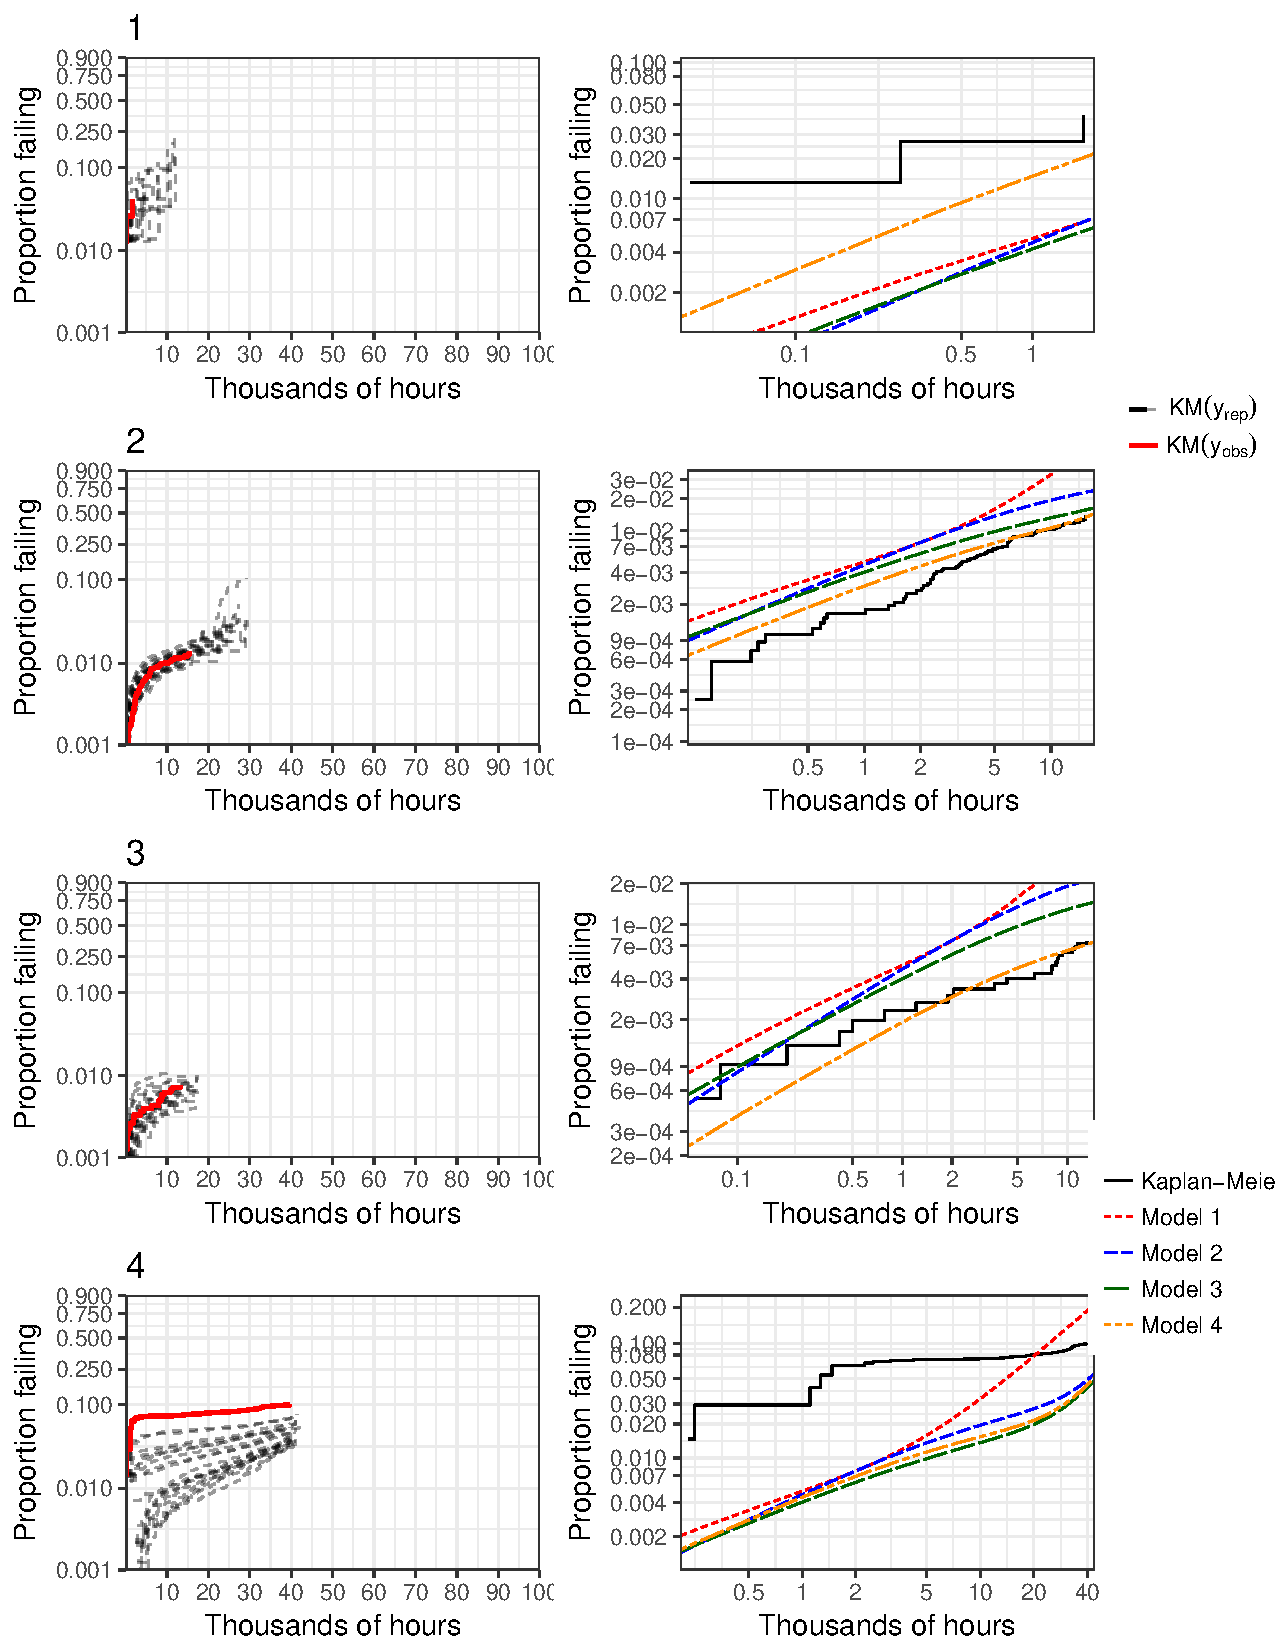
\includegraphics[width=\textwidth]{ppcheck-v2-1.pdf}
\end{figure}
\begin{figure}[H]
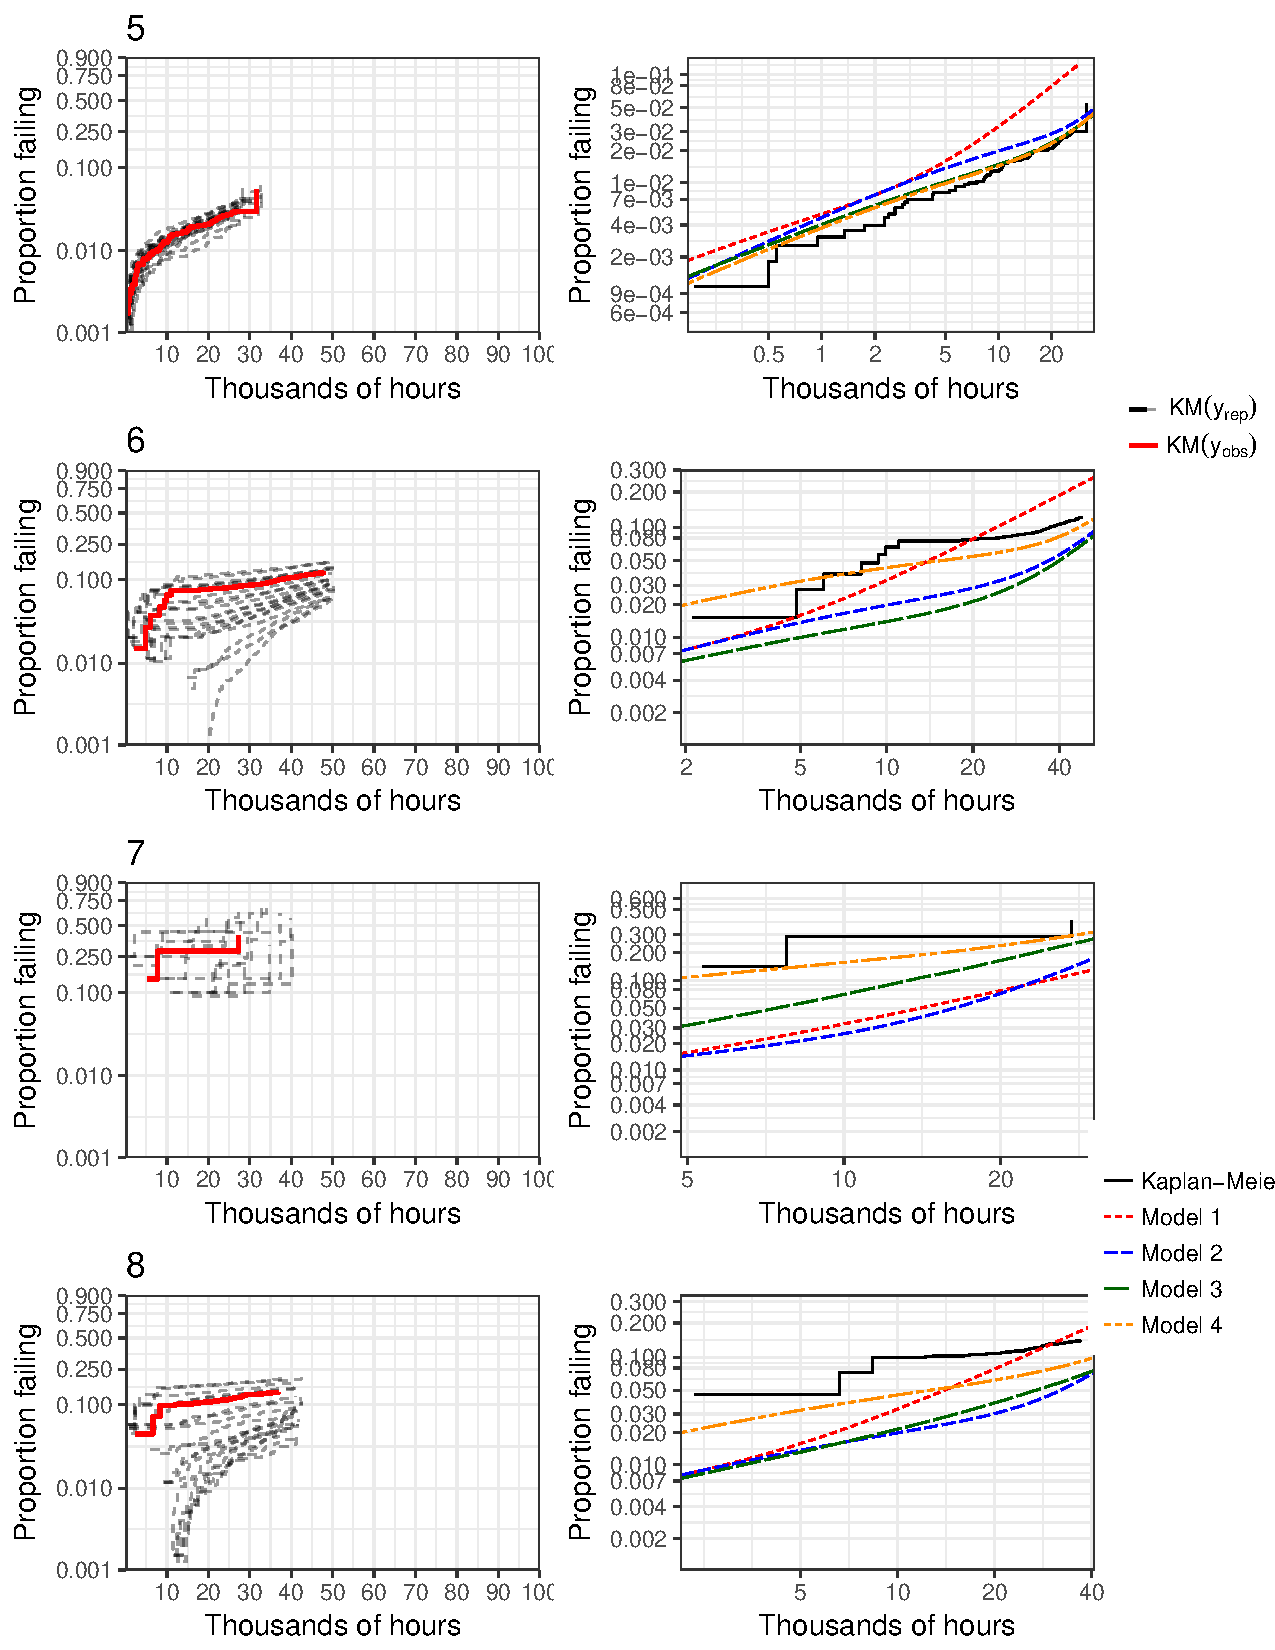
\includegraphics[width=\textwidth]{ppcheck-v2-2}
\end{figure}
\begin{figure}[H]
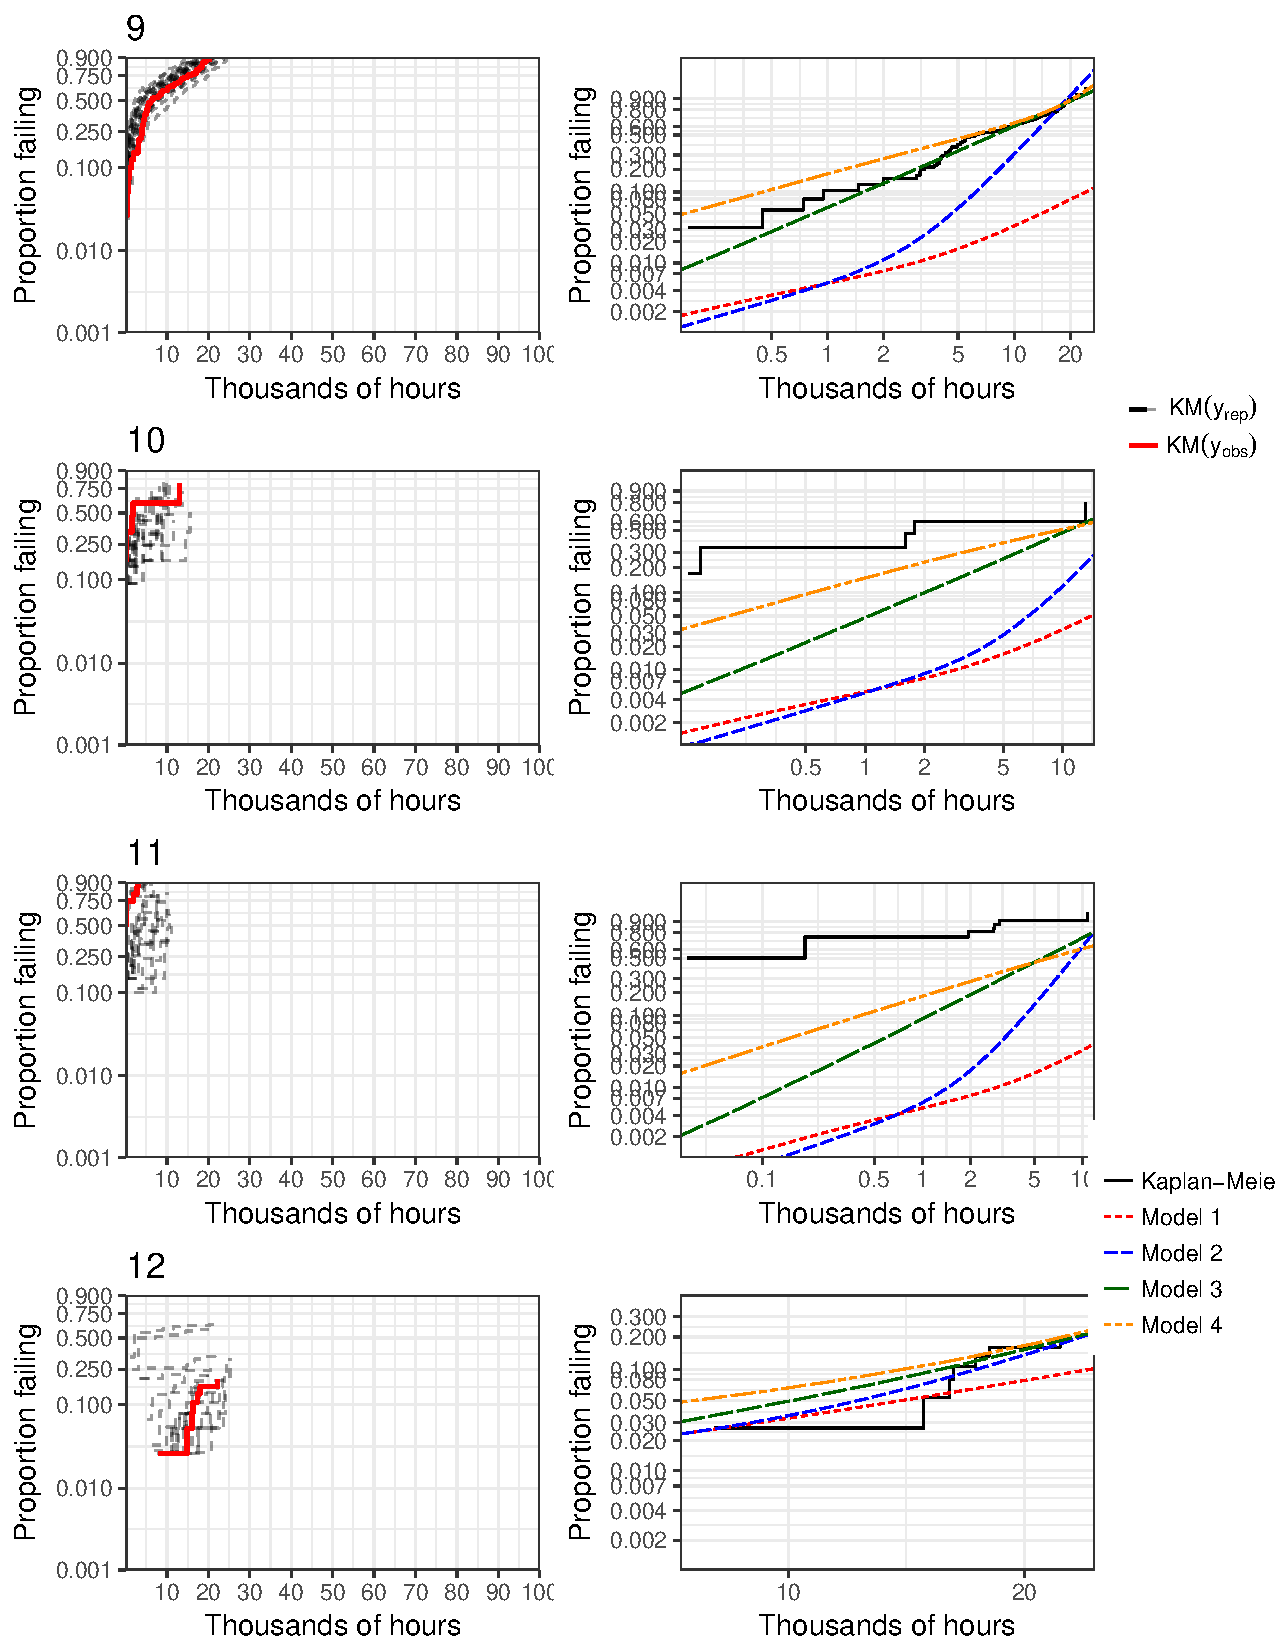
\includegraphics[width=\textwidth]{ppcheck-v2-3.pdf}
\end{figure}
\begin{figure}[H]
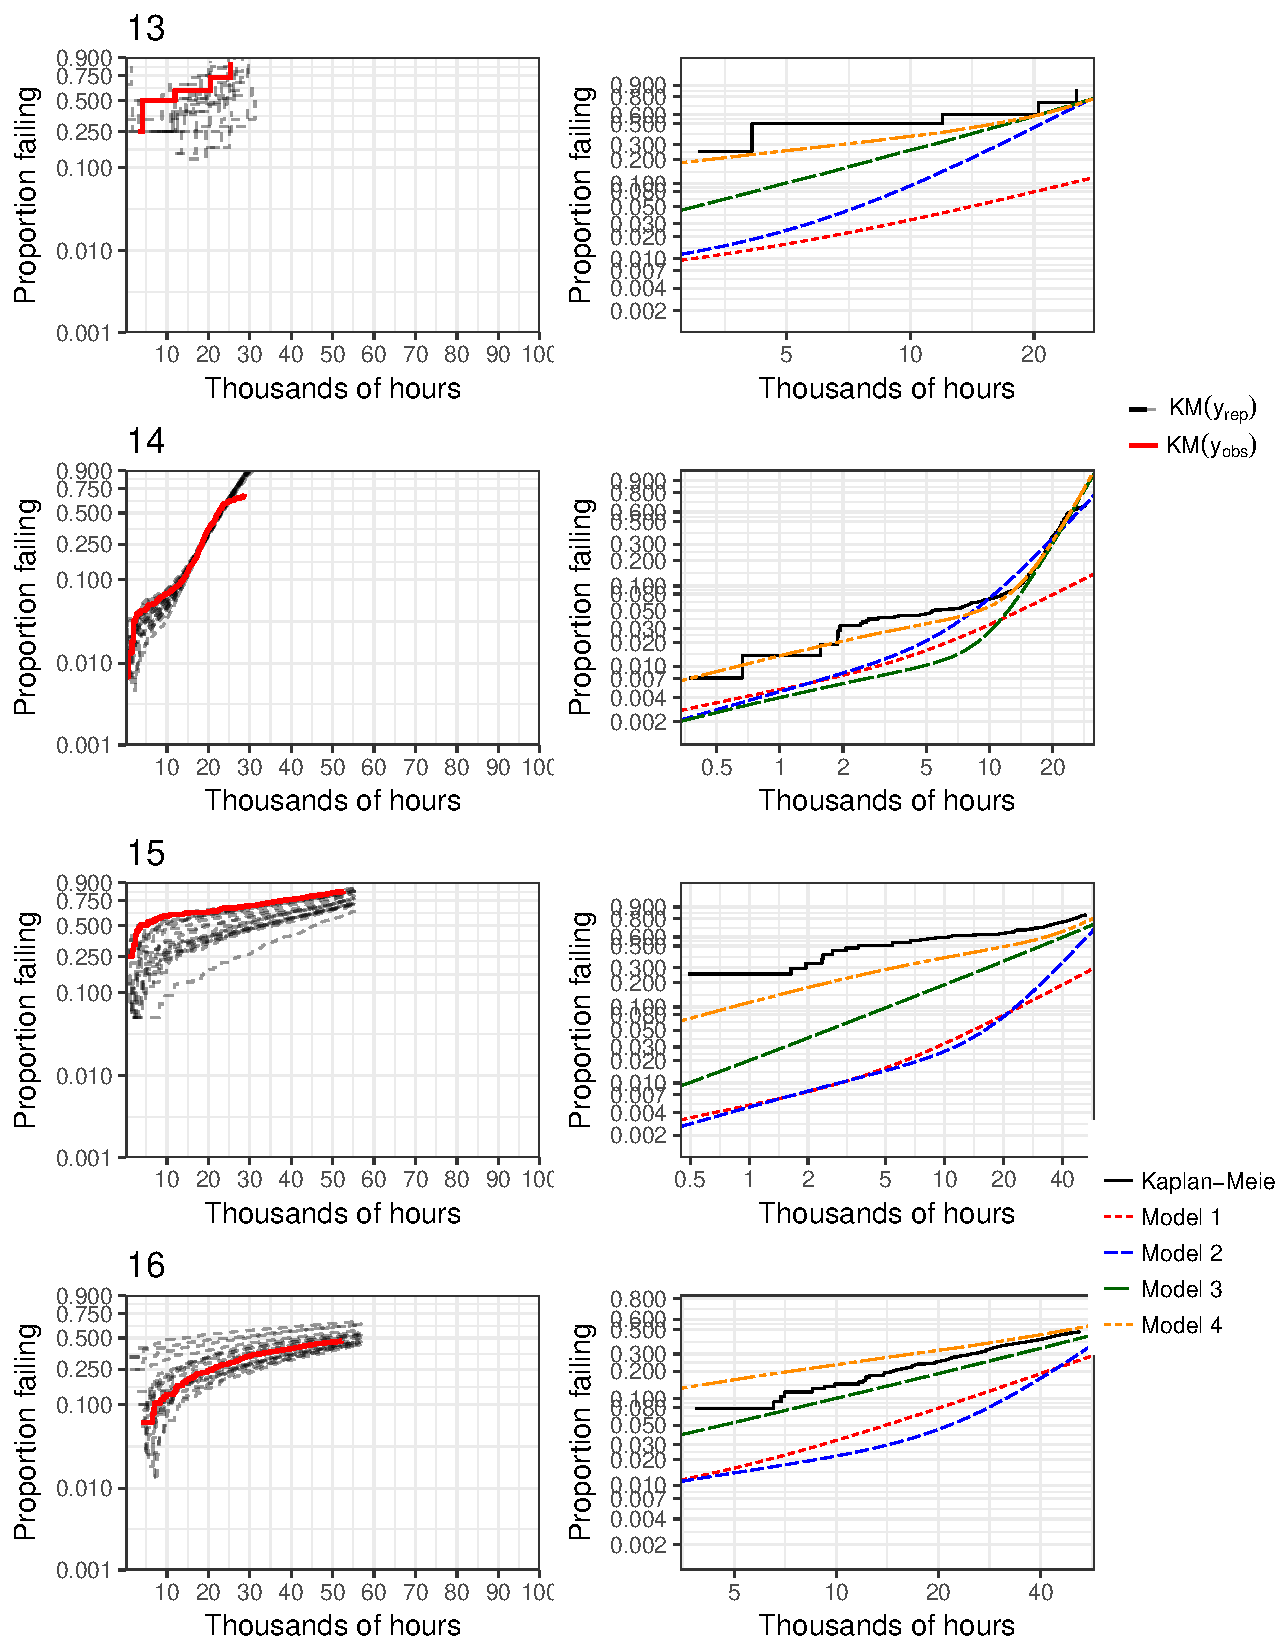
\includegraphics[width=\textwidth]{ppcheck-v2-4.pdf}
\end{figure}
\begin{figure}[H]
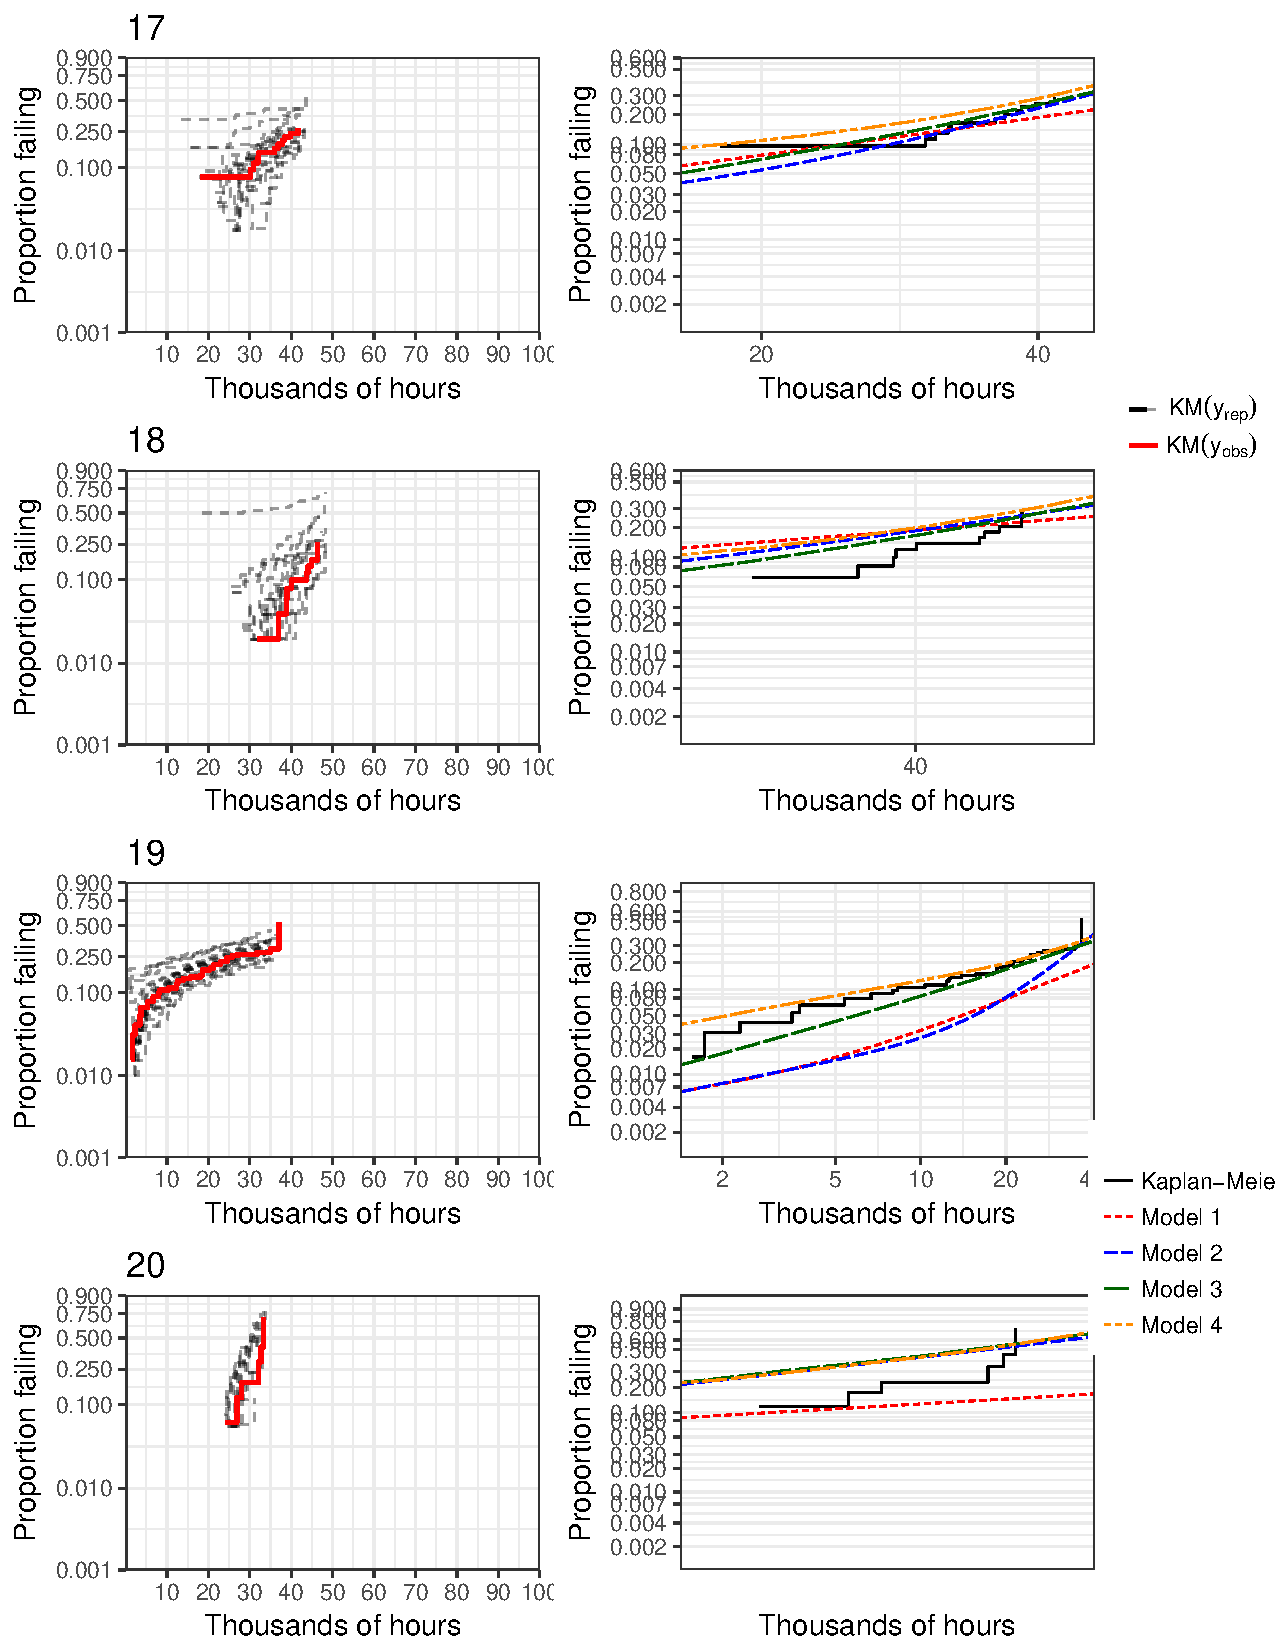
\includegraphics[width=\textwidth]{ppcheck-v2-5.pdf}
\end{figure}
\begin{figure}[H]
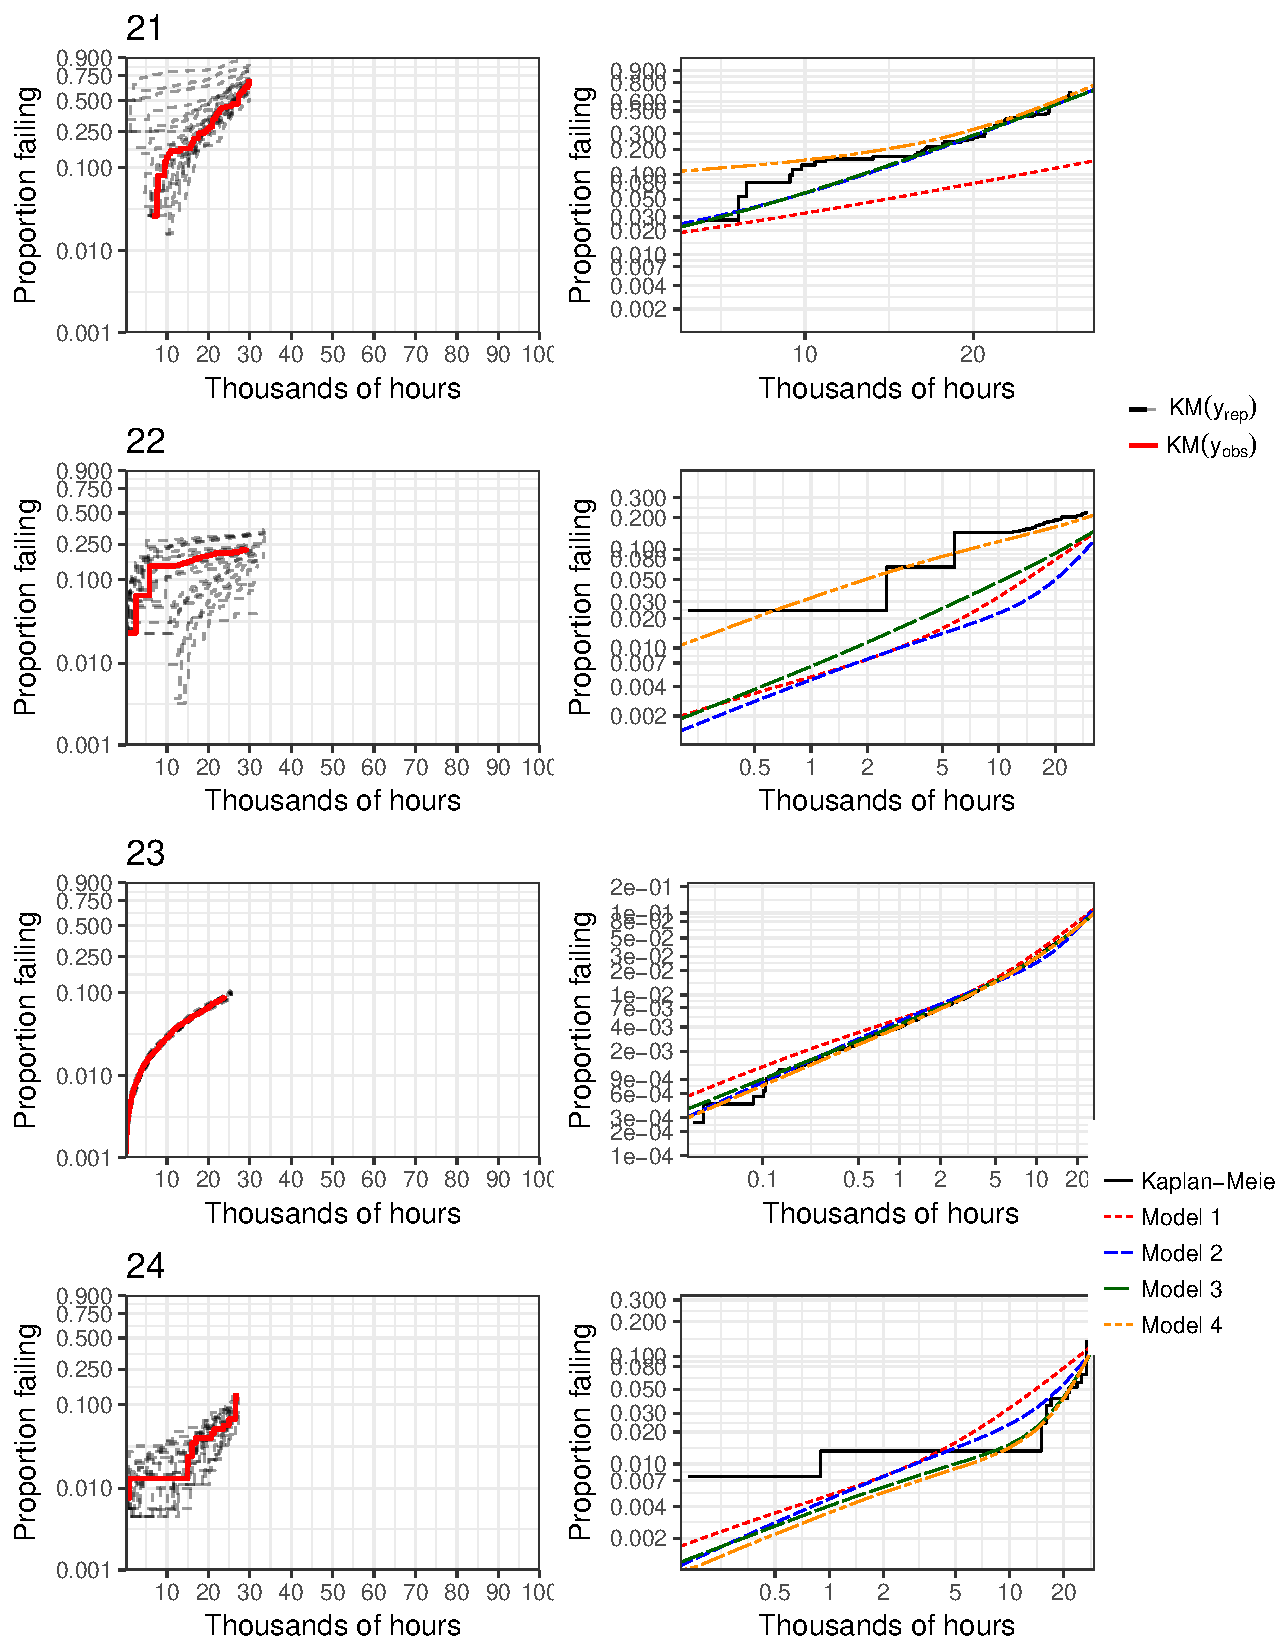
\includegraphics[width=\textwidth]{ppcheck-v2-6.pdf}
\end{figure}
\begin{figure}[H]
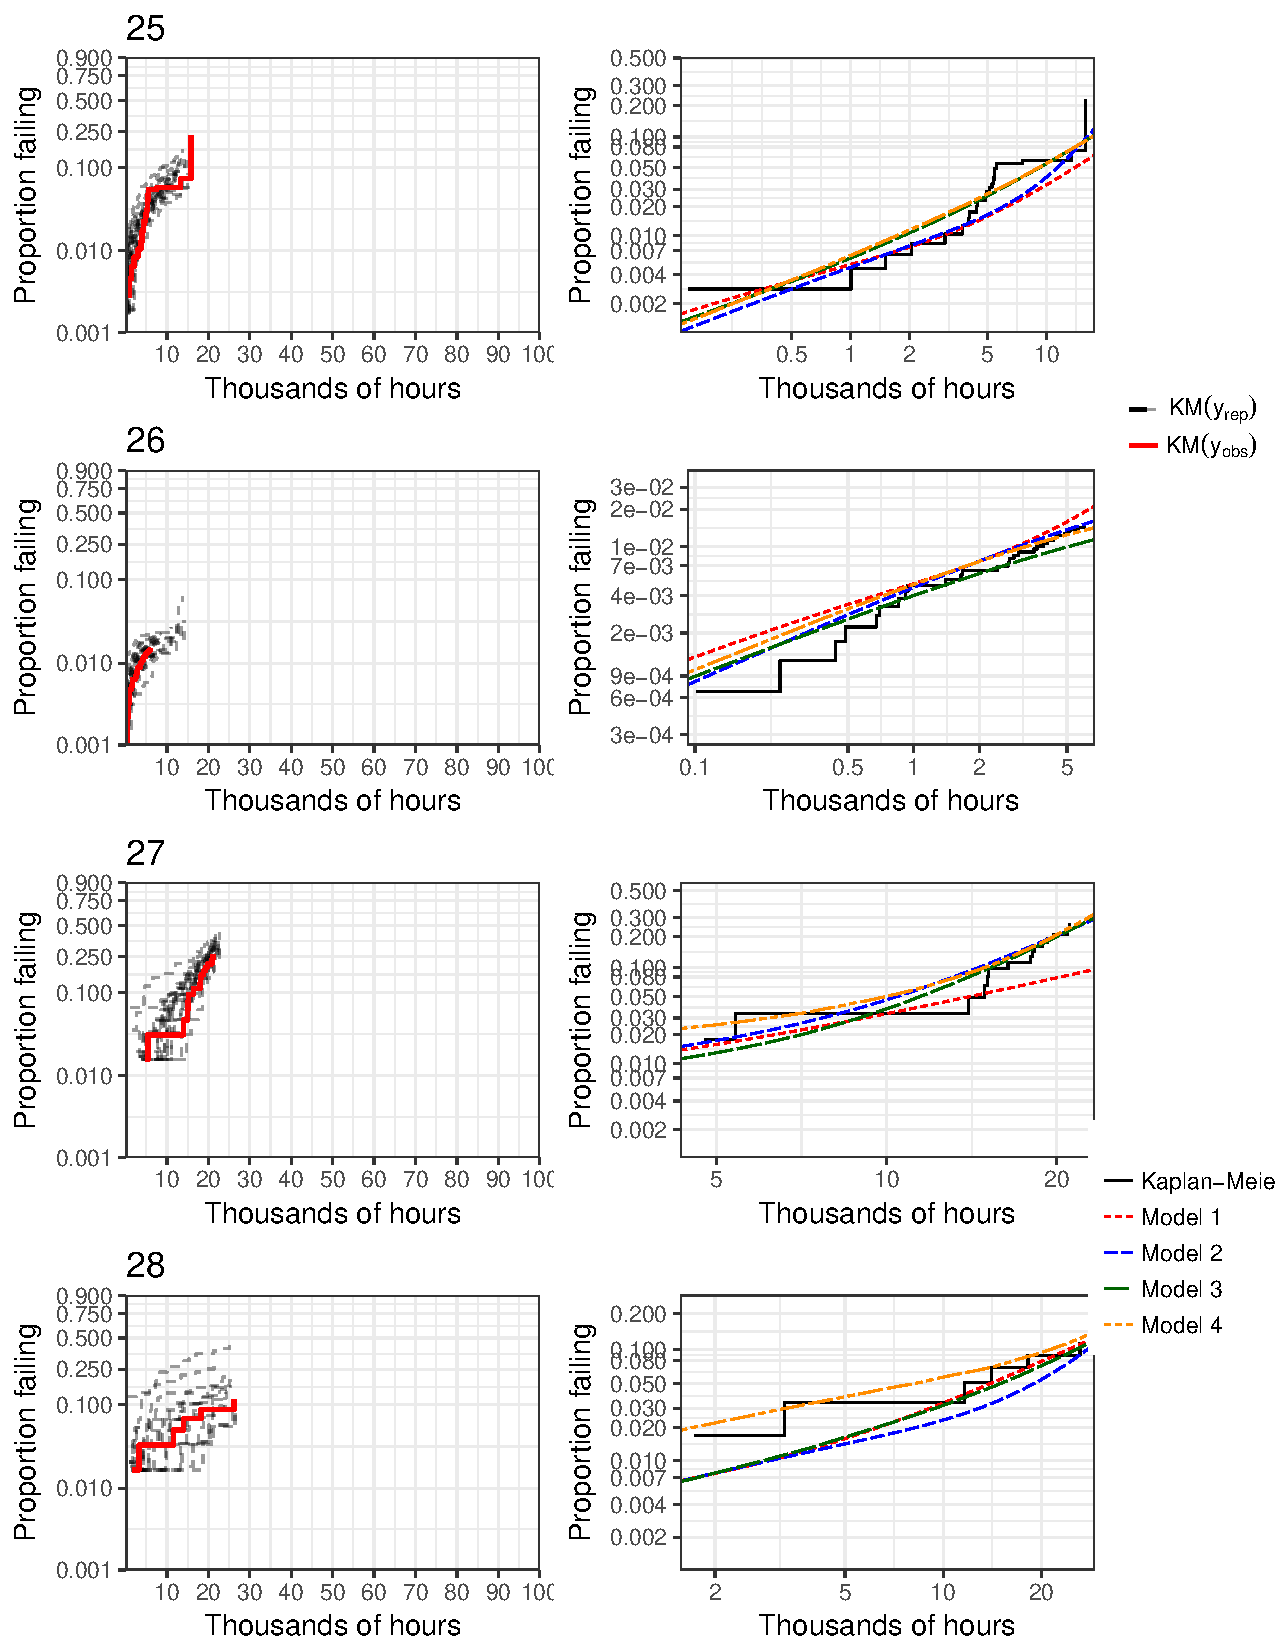
\includegraphics[width=\textwidth]{ppcheck-v2-7.pdf}
\end{figure}
\begin{figure}[H]
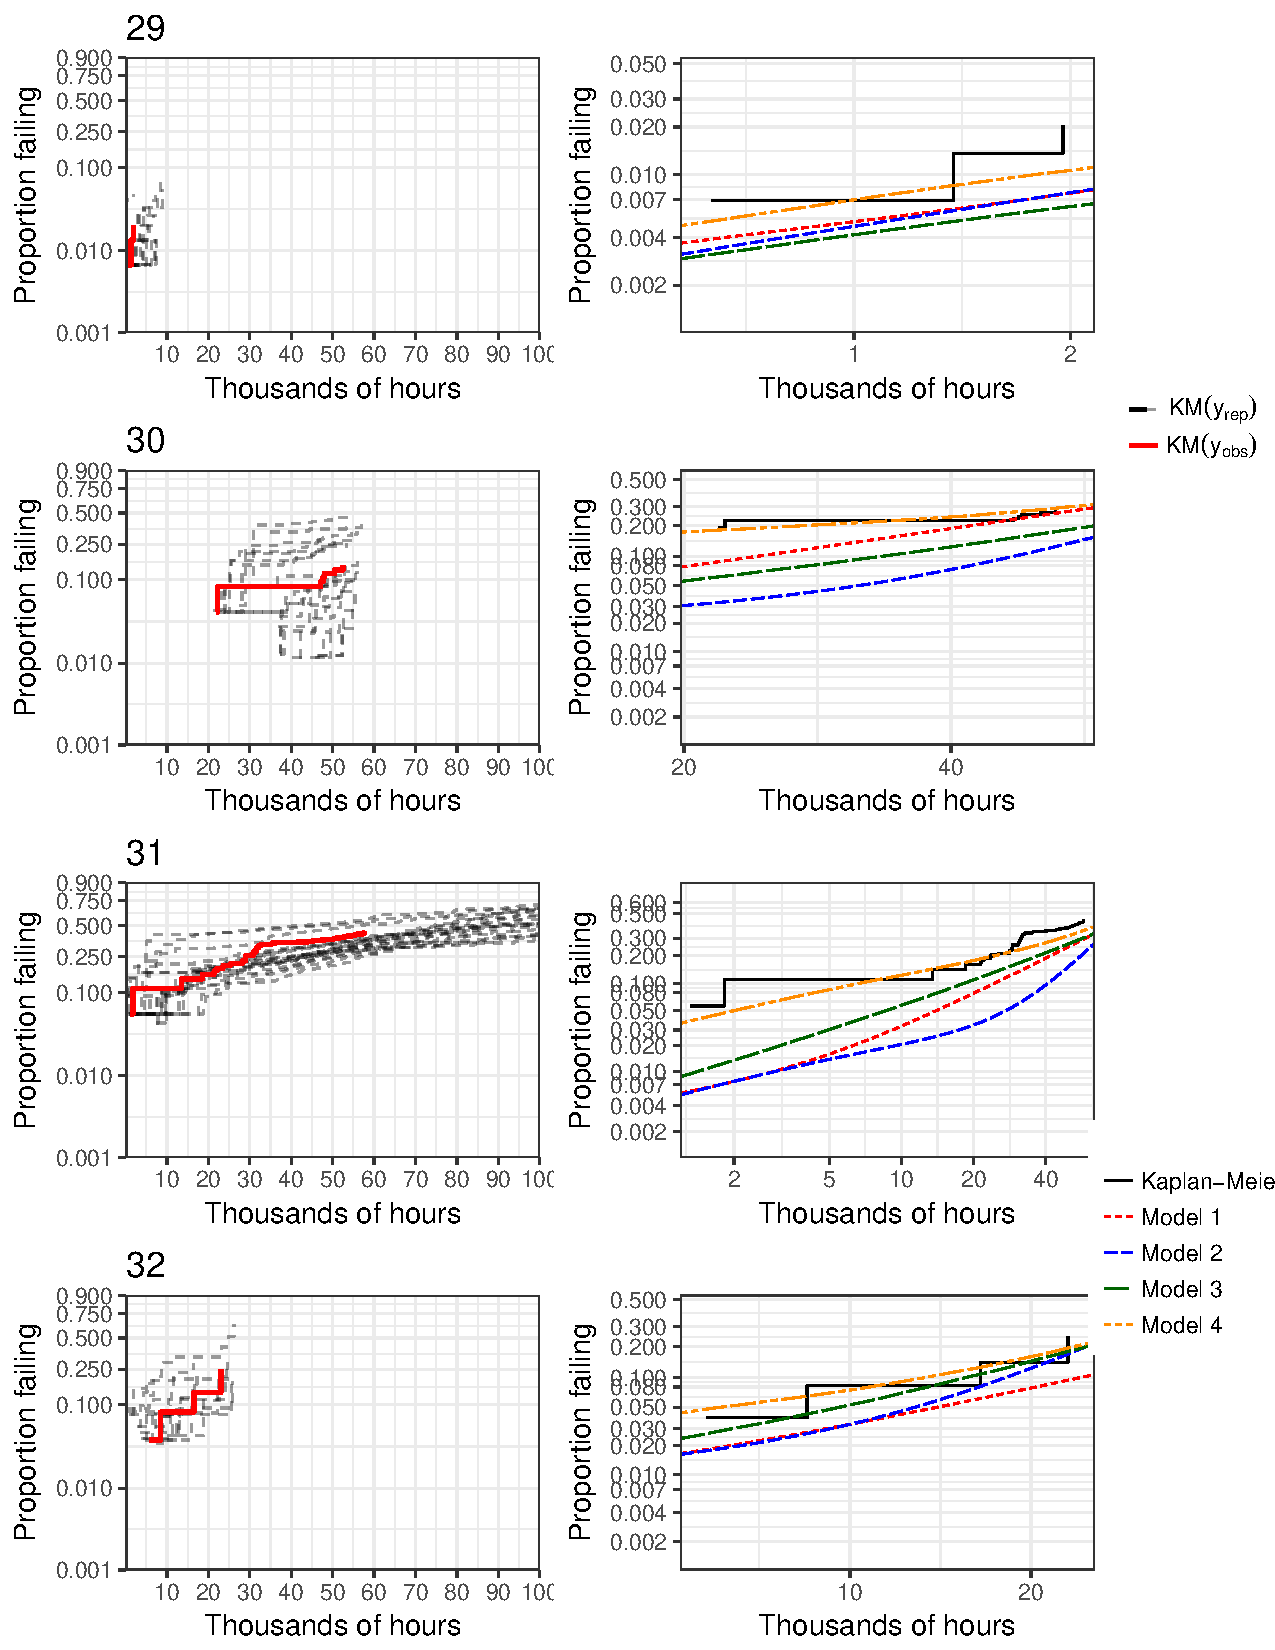
\includegraphics[width=\textwidth]{ppcheck-v2-8.pdf}
\end{figure}
\begin{figure}[H]
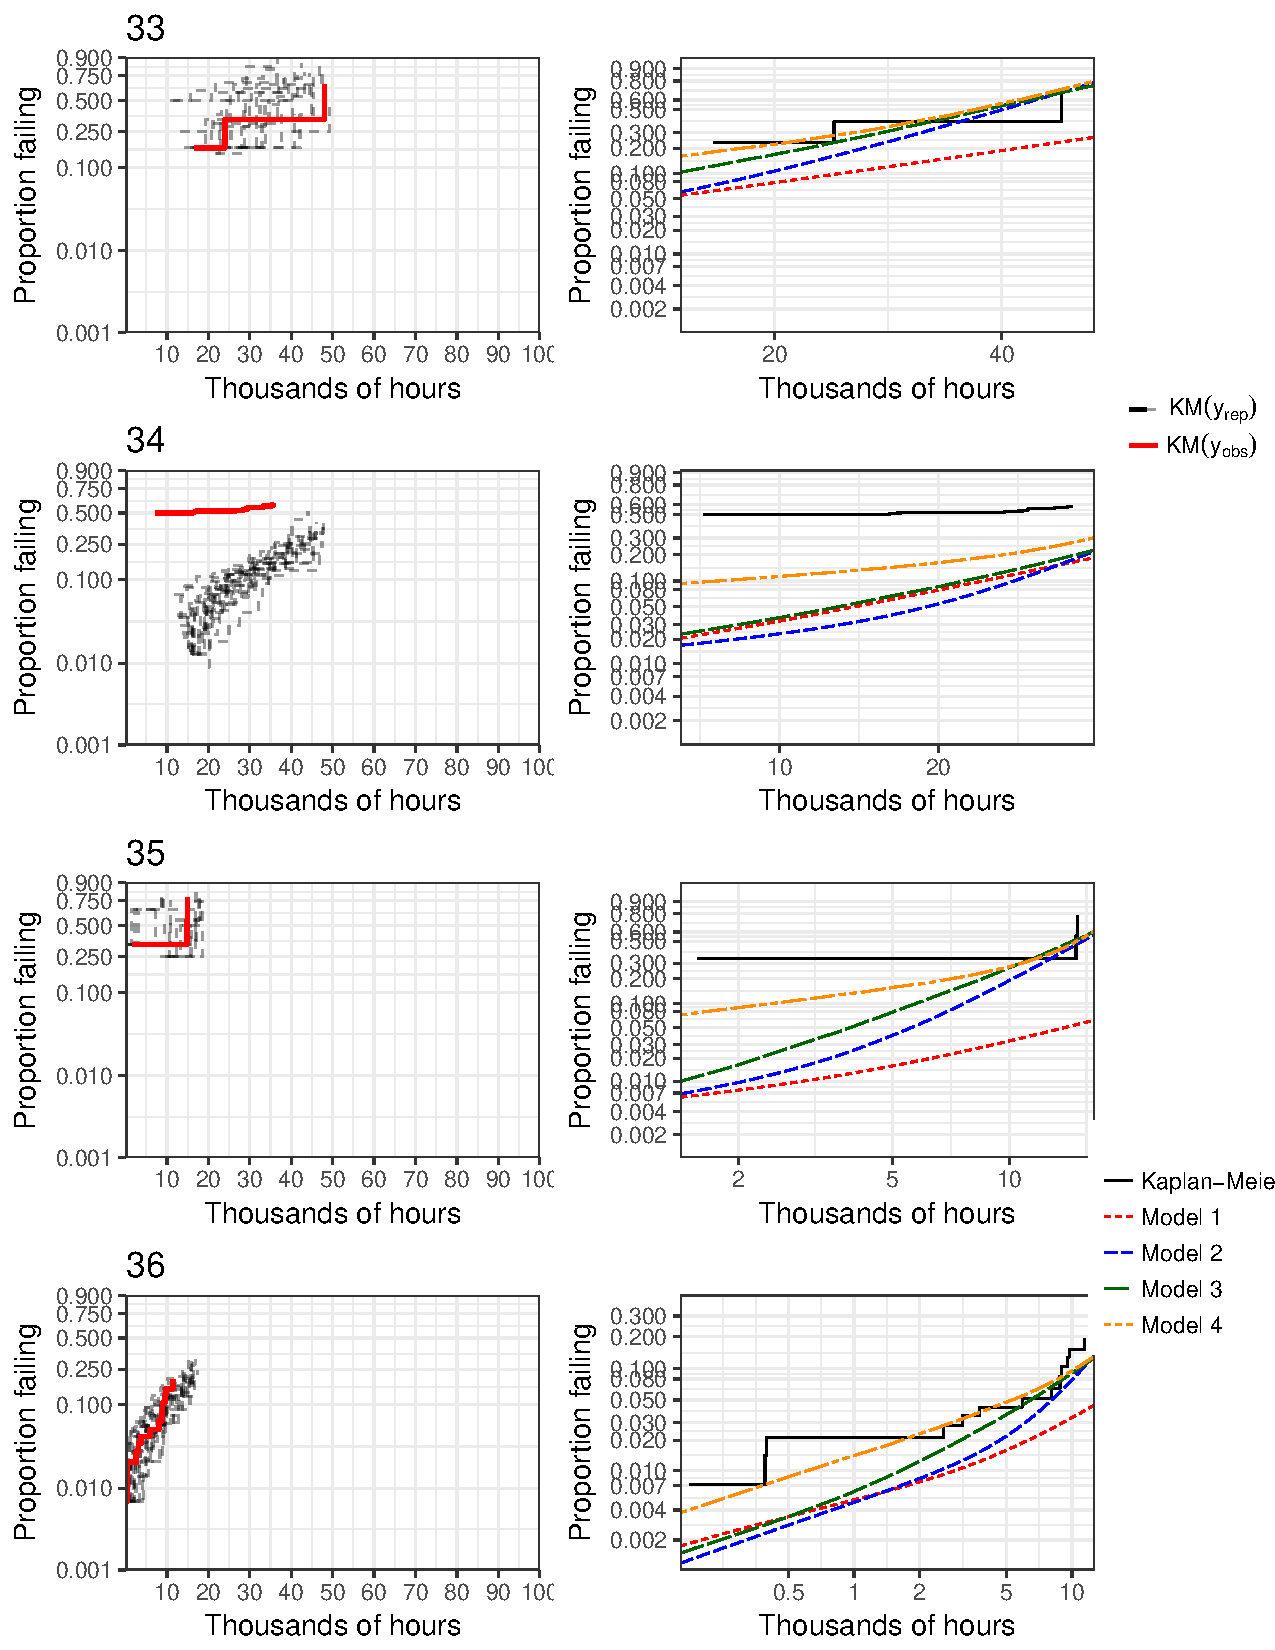
\includegraphics[width=\textwidth]{ppcheck-v2-9.pdf}
\end{figure}
\begin{figure}[H]
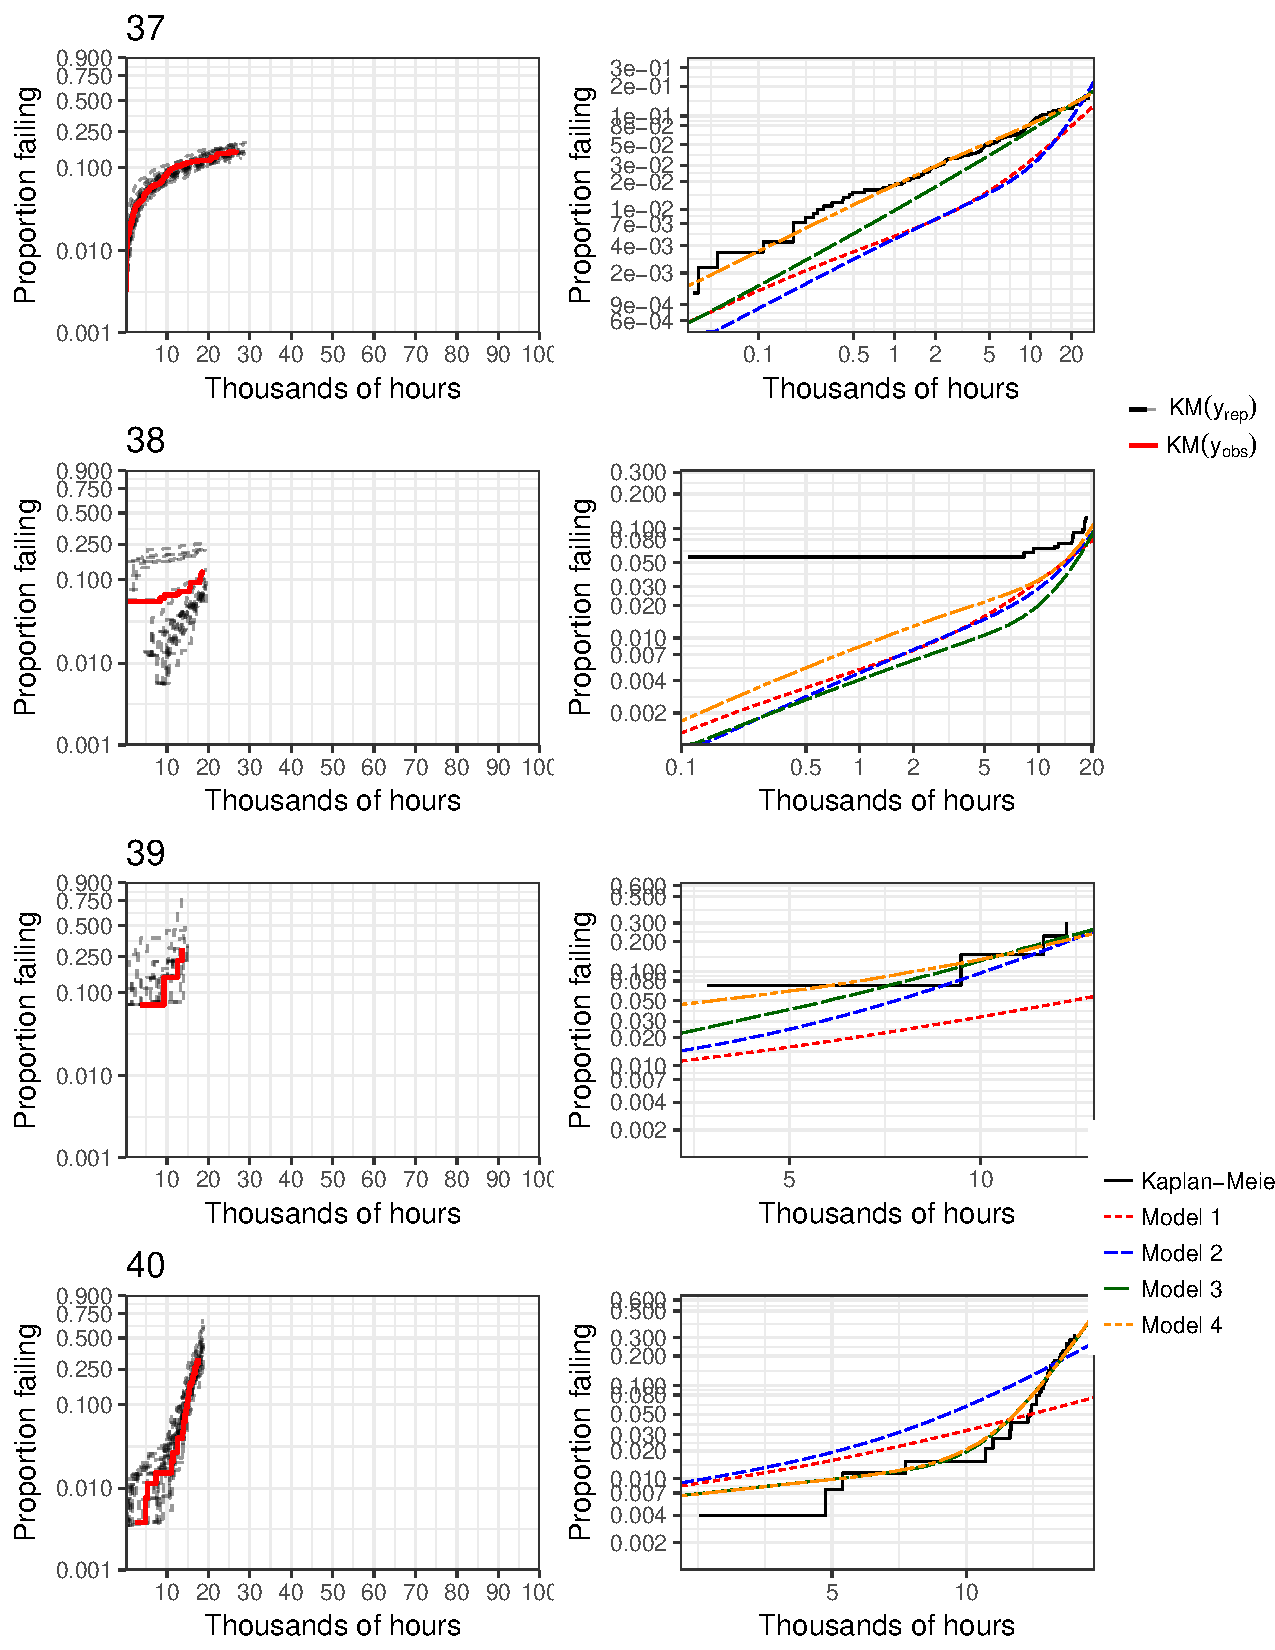
\includegraphics[width=\textwidth]{ppcheck-v2-10.pdf}
\end{figure}
\begin{figure}[H]
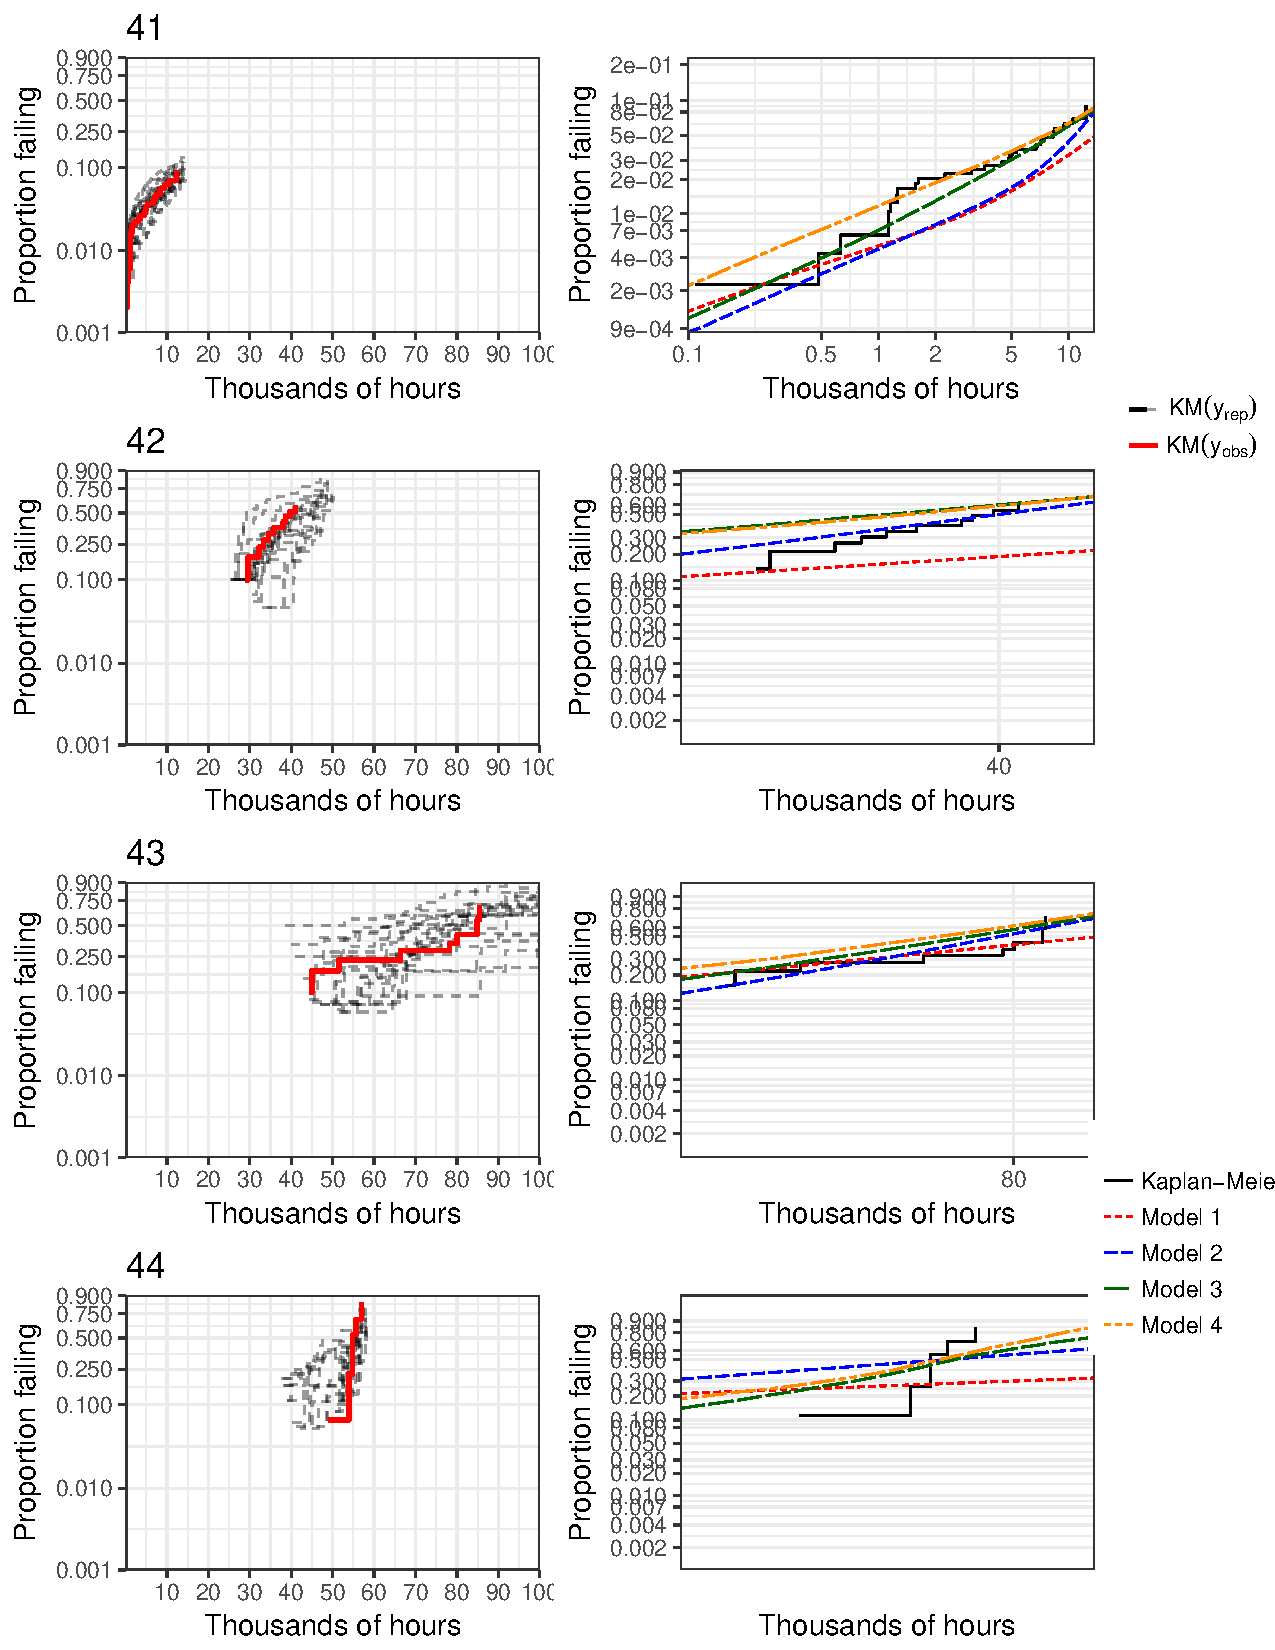
\includegraphics[width=\textwidth]{ppcheck-v2-11.pdf}
\end{figure}
\clearpage

\end{document}